\documentclass{fizykalab}

% Ustawienia do tabelki (uzupełnij według potrzeb)
\wydzial{WI}
\autorjeden{Dawid Komęza}
\autordwa{Magdalena Śmietana}
\rok{II}
\grupa{14}
\zespol{2}
\temat{Wahadło matematyczne - opracowanie danych pomiarowych}
\nrcwiczenia{0}
\datawykonania{09.10.2025}
\dataoddaniajeden{10.11.2025}
\zwrotdopoprawy{}
\dataoddaniadwa{}
\datazaliczenia{}

\begin{document}

\maketitle

\section{Cel ćwiczenia}

Celem ćwiczenia jest praktyczne opanowanie metod opracowania danych
eksperymentalnych na przykładzie wahadła matematycznego oraz wyznaczenie
przyspieszenia ziemskiego \( g \). W szczególności dążymy do:

\begin{itemize}
  \item identyfikacji i odrzucania wyników obarczonych błędem grubym
    (np. reguła \(3\sigma\)),
  \item wyznaczenia niepewności typu~A (na podstawie rozrzutu \(T_i\))
    i typu~B (m.in. odczyt długości \(l\)),
  \item zastosowania prawa przenoszenia niepewności i wyznaczenia
    niepewności rozszerzonej \(U\) (dla \(k \approx 2\)),
  \item graficznej analizy danych: wykonania wykresów \(T(l)\) oraz
    zlinearyzowanego \(T^2(l)\),
  \item dopasowania prostej metodą najmniejszych kwadratów (przez początek
    układu) i oceny jakości dopasowania na podstawie reszt,
  \item wyznaczenia \( g \) dwiema drogami:
    \begin{itemize}
      \item
        (i) z serii pomiarów \(T\) dla ustalonego \(l\),
      \item
        (ii) z nachylenia prostej w zależności \(T^2(l)\),
    \end{itemize}
    oraz porównania wyniku z wartością dla Krakowa
    \( g_{\text{ref}}=\SI{9.811}{\meter\per\second\squared} \)
    w granicach \(U\),
  \item wskazania dominujących źródeł niepewności i potencjalnych
    systematyk (np. dokładność \(l\), reakcja mierzącego).
\end{itemize}

\pagebreak

\section{Wstęp teoretyczny}

Wahadło proste (matematyczne) to idealizowany układ fizyczny
składający się z punktu materialnego o masie \( m \), zawieszonego
na nieważkiej i nierozciągliwej nici o długości \( l \).
Ciężarek wykonuje drgania w płaszczyźnie pionowej
pod wpływem siły ciężkości w polu grawitacyjnym
o przyspieszeniu \( g \).

Dla niewielkich wychyleń kątowych, zwykle nieprzekraczających
\(3^\circ\!-\!5^\circ\), przybliżenie
\(\sin \theta \approx \theta\) pozwala traktować ruch wahadła
jako harmoniczny prosty. Równanie ruchu ma wtedy postać:
\[
  \ddot{\theta} + \frac{g}{l}\theta = 0,
\]
które opisuje drgania o okresie
\[
  T = 2\pi\sqrt{\frac{l}{g}}.
\]
W tym przybliżeniu okres drgań nie zależy od amplitudy,
masy ciężarka ani od kąta wychylenia, lecz jedynie od długości
wahadła i wartości przyspieszenia ziemskiego.

\vspace{1em}
Po podniesieniu równania do kwadratu otrzymujemy postać liniową:
\[
  T^2 = \frac{4\pi^2}{g}\,l,
\]
co oznacza, że wykres zależności \(T^2(l)\) powinien być prostą
przechodzącą przez początek układu współrzędnych.
Nachylenie tej prostej \(a = 4\pi^2/g\) umożliwia zatem
eksperymentalne wyznaczenie wartości \(g\).

\vspace{1em}
Długość wahadła \( l \) interpretujemy jako odległość od punktu
zawieszenia nici do środka ciężkości ciężarka.
Aby ruch zachował charakter harmoniczny,
amplituda drgań powinna być mała; w praktyce przyjmuje się,
że maksymalne wychylenie kątowe nie przekracza \(3^\circ\).

\pagebreak

\section{Wzory}

\subsection{Opracowanie statystyczne pomiarów}

W każdej serii pomiarów uzyskuje się skończoną liczbę wyników
\( x_1, x_2, \ldots, x_n \)
opisujących tę samą wielkość fizyczną (np. okres drgań \(T\)).
Wyniki te obarczone są nieuniknionymi błędami losowymi,
dlatego zamiast pojedynczego odczytu analizuje się całą próbkę
statystycznie.

\vspace{1em}
Średnią arytmetyczną (najlepszy estymator wartości oczekiwanej)
obliczamy jako:
\begin{equation}
  \bar{x} = \frac{1}{n}\sum_{i=1}^{n} x_i.
\end{equation}

Odchylenie standardowe pojedynczego pomiaru (miara rozrzutu wyników)
wyraża się wzorem:
\begin{equation}
  s(x) = \sqrt{\frac{1}{n-1}\sum_{i=1}^{n}
  \left(x_i - \bar{x}\right)^2 }.
\end{equation}

Niepewność typu~A (standardowa niepewność średniej) oblicza się jako:
\begin{equation}
  u_A(x) = \frac{s(x)}{\sqrt{n}}.
\end{equation}
\indent
albo inaczej:
\begin{equation}
  u_A(x) = \sqrt{\frac{\sum_{i=1}^{n} \left(x_i - \bar{x}\right)^2 }{n(n-1)}}.
\end{equation}

\vspace{1em}
Niepewność typu~B określa się na podstawie znanego lub przyjętego
rozkładu możliwych wartości (np. rozkładu prostokątnego dla odczytu
z przyrządu).
Jeśli przyrząd ma działkę elementarną \(\Delta\),
a półzakres możliwego błędu wynosi \(\Delta/2\),
to dla rozkładu prostokątnego:
\begin{equation}
  u_B(x) = \frac{\Delta}{\sqrt{3}}.
\end{equation}

Całkowitą standardową niepewność pomiaru (złożoną)
otrzymujemy z niezależnych niepewności typu A i B:
\begin{equation}
  u_c(x) = \sqrt{u_A^2(x) + u_B^2(x)}.
\end{equation}

Dla przedstawienia końcowego wyniku stosuje się
\emph{niepewność rozszerzoną}
\begin{equation}
  U(x) = k\,u_c(x),
\end{equation}
gdzie \( k \) jest współczynnikiem rozszerzenia zależnym od
pożądanego poziomu pewności.
Najczęściej przyjmuje się \( k = 2 \) lub \( k = 3 \), co odpowiada
odpowiednio poziomom pewności około \(95\,\%\) i \(99.7\,\%\).

\vspace{1em}
Jeśli któryś z wyników \(\,x_i\,\) spełnia warunek
\(|x_i - \bar{x}| > 3\,s(x)\),
to można go uznać za \emph{błąd gruby}
i odrzucić na podstawie tzw. \emph{reguły trzech sigma}.
Po odrzuceniu takich punktów obliczenia \(\bar{x}\)
i \(s(x)\) należy powtórzyć.

\subsection{Wzory fizyczne i przenoszenie niepewności}

Wahadło matematyczne o długości \( l \) drgające w polu grawitacyjnym
o przyspieszeniu \( g \) ma dla małych kątów wychylenia okres drgań
określony zależnością:
\begin{equation}
  T = 2\pi \sqrt{\frac{l}{g}}.
\end{equation}
Po przekształceniu otrzymujemy wzór pozwalający obliczyć
przyspieszenie ziemskie z pomiaru okresu \( T \) i długości \( l \):
\begin{equation}
  g = \frac{4\pi^2\,l}{T^2}.
\end{equation}

Dla pomiarów wykonywanych wielokrotnie dla kilku różnych długości
wahadła można zlinearyzować zależność przez podniesienie do kwadratu:
\begin{equation}
  T^2 = \frac{4\pi^2}{g}\,l,
\end{equation}
czyli \( T^2(l) \) jest funkcją liniową o współczynniku nachylenia
\begin{equation}
  a = \frac{4\pi^2}{g}.
\end{equation}
Z nachylenia prostej wyznaczonego metodą najmniejszych kwadratów można
więc obliczyć:
\begin{equation}
  g = \frac{4\pi^2}{a}.
\end{equation}

\subsubsection*{Przenoszenie niepewności}

Wpływ niepewności pomiaru \( l \) i \( T \) na niepewność \(\,g\)
określa \emph{prawo przenoszenia niepewności}:
\begin{equation}
  u_c(g) =
  \sqrt{
    \left(\frac{\partial g}{\partial l}u(l)\right)^2 +
    \left(\frac{\partial g}{\partial T}u(T)\right)^2
  }.
\end{equation}

\vspace{1em} \noindent
Z analizy wzoru \( g(l,T) = 4\pi^2l/T^2 \) wynika:
\begin{equation}
  \frac{\partial g}{\partial l} = \frac{4\pi^2}{T^2},
  \qquad
  \frac{\partial g}{\partial T} = -\frac{8\pi^2\,l}{T^3}.
\end{equation}

\vspace{1em} \noindent
Po podstawieniu dostajemy:
\begin{equation}
  u_c(g) = \sqrt{
    \left(\frac{4\pi^2}{T^2}u(l)\right)^2 +
  \left(\frac{8\pi^2\,l}{T^3}u(T)\right)^2 }.
\end{equation}

\vspace{1em} \noindent
W postaci względnej wygodniej zapisać:
\begin{equation}
  \frac{u_c(g)}{g} =
  \sqrt{
    \left(\frac{u(l)}{l}\right)^2 +
  \left(2\,\frac{u(T)}{T}\right)^2 }.
\end{equation}

\vspace{1em} \noindent
Niepewność rozszerzoną przyjmujemy dla współczynnika rozszerzenia
\(k = 2\):
\begin{equation}
  U(g) = k\,u_c(g) \approx 2\,u_c(g),
\end{equation}
co odpowiada przedziałowi pewności na poziomie ok.~95 \%.

\subsubsection*{Ocena zgodności z wartością tablicową}

Wartość tablicowa przyspieszenia ziemskiego dla Krakowa wynosi
\[
  g_{\text{ref}} = \SI{9.811}{\meter\per\second\squared}.
\]
Wynik pomiarów uznaje się za zgodny z wartością tablicową,
jeżeli spełniony jest warunek:
\begin{equation}
  |g - g_{\text{ref}}| \le U(g).
\end{equation}

\section{Aparatura pomiarowa}

Do wykonania ćwiczenia wykorzystano klasyczny zestaw wahadła
matematycznego oraz podstawowe przyrządy pomiarowe:

\begin{itemize}
  \item \textbf{Zestaw wahadła prostego} – metalowy ciężarek zawieszony
    na cienkiej, nierozciągliwej nici przymocowanej do wspornika.
    Układ pozwala na regulację długości \(l\) wahadła w szerokim
    zakresie (ok.\ 10 – 30 cm). Nicię traktuje się jako bezmasową,
    a ciężarek jako punkt materialny.
  \item \textbf{Sekundomierz (stoper)} – cyfrowy stoper o rozdzielczości
    \SI{0.01}{\second}. Służy do pomiaru czasu \(t\) wielokrotnej
    liczby \(k\) okresów drgań, aby zmniejszyć wpływ błędu reakcji
    operatora. Pomiar rozpoczyna i kończy się w tej samej fazie ruchu
    (np. w maksymalnym wychyleniu w prawo).
  \item \textbf{Przymiar milimetrowy (linijka)} – używany do wyznaczenia
    długości wahadła \(l\), rozumianej jako odległość od punktu
    zawieszenia nici do środka ciężkości ciężarka. Linijka ma skalę
    co \(\SI{1}{\milli\meter}\), co przekłada się na dokładność
    odczytu: \(\pm\,\SI{0.5}{\milli\meter}\).
\end{itemize}

\begin{figure}[H]
  \centering
  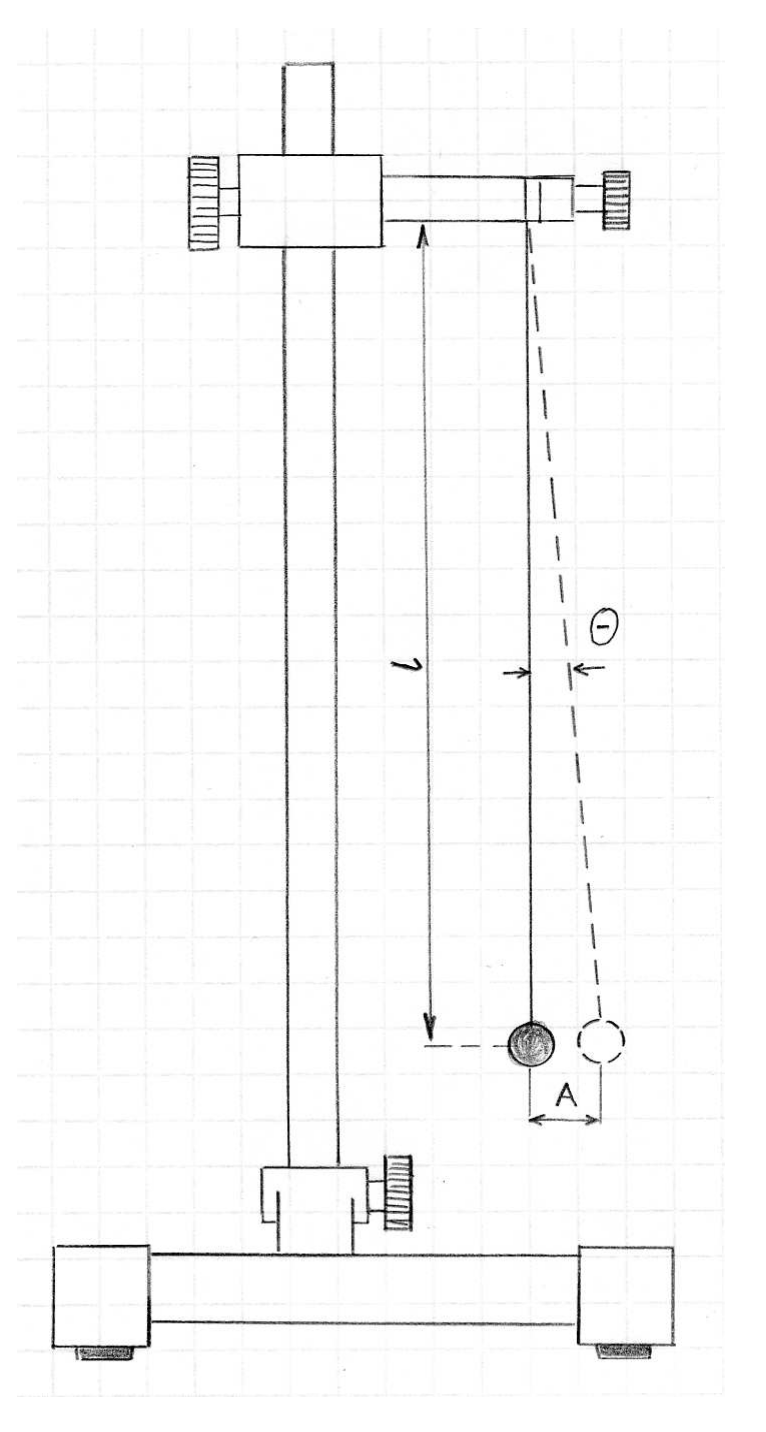
\includegraphics[width=0.65\textwidth]{./wahadlo.png}
  \caption{Schemat zestawu wahadła prostego.
    Długość \(l\) mierzona jest od punktu zawieszenia
  do środka ciężkości ciężarka, amplituda wychylenia \(A = l\,\theta\).}
  \label{fig:wahadlo}
\end{figure}

Podczas pomiaru istotne jest zachowanie powtarzalnych warunków
eksperymentu: minimalnych drgań podstawy, braku przeciągów
i utrzymanie małej amplitudy początkowej. Wyniki pomiarów \(t\)
dla określonego \(k\) przeliczano następnie na okres \(T = t/k\).
\pagebreak

\section{Wyniki dla pojedynczego pomiaru}

Dla ilustracji obliczeń wykonano pojedynczy pomiar okresu drgań dla jednej
z wybranych długości wahadła. Zmierzono, że wahadło miało długość
\[
  l = \SI{190}{\milli\meter} =  \SI{0.29}{\meter}
\]
(z dokładnością \(\pm \SI{2}{\milli\meter} = \pm\SI{0.002}{\meter}\)).
Zmierzono czas \(t\) dla \(k = 10\) okresów, otrzymując:
\[
  t = \SI{11.17}{\second}, \qquad
  T = \frac{t}{k} = \frac{11.17}{10} = \SI{1.117}{\second}.
\]

\subsection{Wyznaczenie przyspieszenia ziemskiego}

Na podstawie zależności \( g = 4\pi^2 l / T^2 \) otrzymano:
\[
  g = \frac{4\pi^2 \cdot 0.290}{(1.117)^2}
  = \SI{9.17}{\meter\per\second\squared}.
\]

\subsection{Niepewności pomiarowe}

Niepewność typu B dla długości:
\[
  u(l) = \frac{0.002}{\sqrt{3}} = \SI{0.00115}{\meter}.
\]

Niepewność standardowa pomiaru okresu (przyjęta na podstawie
dokładności odczytu czasu \(\pm 0.2\,\text{s}\)):
\[
  u(T) = \frac{0.2}{k} = \SI{0.02}{\second}.
\]

Z prawa przenoszenia niepewności:
\[
  \frac{u_c(g)}{g} =
  \sqrt{
    \left(\frac{u(l)}{l}\right)^2 +
  \left(2\frac{u(T)}{T}\right)^2 }
  =
  \sqrt{
    \left(\frac{0.00115}{0.29}\right)^2 +
  \left(2\frac{0.02}{1.117}\right)^2 }
  = 0.036.
\]
\[
  u_c(g) = 0.036 \times 9.17 = \SI{0.33}{\meter\per\second\squared}, \qquad
  U(g) = 2u_c(g) = \SI{0.66}{\meter\per\second\squared}.
\]

\subsection{Wynik końcowy}

\[
  \boxed{
    g = (10.37 \pm 0.66)\,
    \si{\meter\per\second\squared}\quad(k=2)
  }
\]

\subsection{Komentarz}

Wartość \(g = 9,17\,\si{m/s^2}\) jest mniejsza od wartości tablicowej
\(g_\text{ref} = 9.811\,\si{m/s^2}\), ale różnica \( |g - g_\text{ref}| = 0.63 < U(g)\)
oznacza, że wynik jest \textbf{zgodny w granicach niepewności pomiarowej}.
Duża relatywna niepewność (ponad 8 \%) wiąże się z tym, że pomiar opiera się
na pojedynczym odczycie czasu i nie pozwala uśrednić błędów reakcji.
Metoda ta ma charakter poglądowy i służy jedynie do sprawdzenia poprawności
procedury obliczeniowej.
\pagebreak

\section{Wyniki pomiarów dla ustalonej długości linki}

Długość wahadła:
\[
  l = \SI{0.290}{\meter}
  \quad (\text{z~dokładnością } \pm \SI{2}{\milli\meter}),
\]
czyli niepewność typu B:
\[
  u_B(l) = \SI{2}{\milli\meter} = \SI{0.002}{\meter}.
\]

\begin{table}[H]
  \centering
  \caption{Pomiar czasu dla \emph{ustalonej} długości wahadła.}
  \begin{tabular}{cccc}
    \toprule
    Lp. & Liczba okresów \(k\) & Czas \(t\)\,[\si{\second}] & Okres \(T_i = t/k\)\,[\si{\second}] \\
    \midrule
    1 & 10 & 10.41 & 1.041 \\
    2 & 10 & 10.55 & 1.055 \\
    3 & 10 & 10.56 & 1.056 \\
    4 & 10 & 10.57 & 1.057 \\
    5 & 10 & 10.76 & 1.076 \\
    6 & 10 & 10.66 & 1.066 \\
    7 & 10 & 10.62 & 1.062 \\
    8 & 10 & 10.74 & 1.074 \\
    9 & 10 & 10.54 & 1.054 \\
    10 & 10 & 10.49 & 1.049 \\
    \bottomrule
  \end{tabular}
  \label{tab:wahadlo_fixed}
\end{table}

\subsection{Opracowanie wyników}

Średnia:
\[
  \bar{T} = \SI{1.059}{\second}.
\]

Odchylenie standardowe:
\[
  s(T) = \sqrt{\frac{\sum_{i=1}^{n}
  \left(T_i - \bar{T}\right)^2}{n-1}} =
  \sqrt{\frac{\sum_{i=1}^{10}
  \left(T_i - 1.059\right)^2}{9}} = \SI{0.010}{\second}
\]

\[
  u_A(T) = \frac{s(T)}{\sqrt{10}} = \SI{0.0034}{\second}
\]

Żaden z wyników nie przekracza warunku \(|T_i - \bar{T}| > 3s(T)\),
więc wszystkie punkty uznano za poprawne.

\subsection{Wyznaczenie przyspieszenia ziemskiego}

Z wzoru
\[
  g = \frac{4\pi^2 l}{\bar{T}^2}
\]
otrzymujemy:
\[
  g = \frac{4\pi^2 \cdot 0.290}{(1.059)^2}
  = \SI{10.21}{\meter\per\second\squared}.
\]

\subsection{Niepewność złożona i rozszerzona}

Prawo przenoszenia niepewności:
\[
  \frac{u_c(g)}{g} =
  \sqrt{
    \left(\frac{u(l)}{l}\right)^2 +
    \left(2\frac{u(T)}{T}\right)^2
  }
  =
  \sqrt{
    \left(\frac{0.002}{0.290}\right)^2 +
    \left(\frac{2 \cdot 0.0034}{1.059}\right)^2
  }
  = 0.0094.
\]
\[
  u_c(g) = 0.0094 \times 10.21 = \SI{0.096}{\meter\per\second\squared}.
\]
\[
  U(g) = 2u_c(g) = \SI{0.19}{\meter\per\second\squared}.
\]

\subsection{Wynik końcowy i ocena zgodności}

\[
  \boxed{
    g = (10.21 \pm 0.19)\,
    \si{\meter\per\second\squared}\quad(k=2)
  }
\]

Dla wartości tablicowej \( g_\text{ref} = 9.811\,
\si{\meter\per\second\squared} \) różnica wynosi
\(|g - g_\text{ref}| = 0.32 > U(g)\),
co oznacza, że wynik \textbf{nie jest zgodny} z wartością tablicową w granicach
niepewności rozszerzonej.

\subsection{Komentarz do wyniku}

Otrzymany wynik \( g = (10.21 \pm 0.19)\,\si{m/s^2} \)
jest nieznacznie wyższy od wartości tablicowej
\( g_\text{ref} = 9.811\,\si{m/s^2} \)
i nie mieści się w granicach niepewności rozszerzonej.
Różnica może wynikać z obecności błędów systematycznych,
w szczególności:
\begin{itemize}
  \item niedokładnego wyznaczenia długości wahadła -
    długość rzeczywista mogła być większa od zmierzonej,
    co mogło być spowodowane na przykład niedokładnym wyznaczeniem
    środka ciężkości ciężarka,
  \item zbyt dużej amplitudy wychylenia lub niedokładnego
    momentu zatrzymania stopera,
  \item braku idealnego ruchu w jednej płaszczyźnie oraz
    niewielkiego tarcia w punkcie zawieszenia.
\end{itemize}
Pomimo niezgodności ilościowej,
wynik znajduje się w rozsądnym przedziale wartości
i pokazuje poprawną zależność okresu od długości wahadła,
co potwierdza poprawność jakościową przeprowadzonego eksperymentu.

\pagebreak

\section{Wyniki pomiarów dla zmiennej długości linki}

W drugiej części ćwiczenia badano zależność okresu drgań wahadła
od jego długości. Dla każdej długości \(l\) zmierzono czas \(t\)
odpowiadający \(k = 10\) pełnym okresom, a następnie obliczono
\(T_i = t/k\) oraz \(T_i^2\).
Długości wahadła mieściły się w zakresie
od \SI{120}{\milli\meter} do \SI{355}{\milli\meter}.

\begin{table}[H]
  \centering
  \caption{Pomiar okresu drgań dla różnych długości wahadła.}
  \begin{tabular}{cccccc}
    \toprule
    Lp. & \(l\)\,[\si{\milli\meter}] &
    \(k\) & \(t\)\,[\si{\second}] &
    \(T_i\)\,[\si{\second}] & \(T_i^2\)\,[\si{\second\squared}]\\
    \midrule
    1 & 355 & 10 & 11,81 & 1,181 & 1,395 \\
    2 & 330 & 10 & 11,20 & 1,120 & 1,254 \\
    3 & 290 & 10 & 10,66 & 1,066 & 1,136 \\
    4 & 247 & 10 &  9,69 & 0,969 & 0,939 \\
    5 & 208 & 10 &  8,92 & 0,892 & 0,796 \\
    6 & 180 & 10 &  8,22 & 0,822 & 0,676 \\
    7 & 160 & 10 &  7,73 & 0,773 & 0,598 \\
    8 & 145 & 10 &  7,30 & 0,730 & 0,533 \\
    9 & 130 & 10 &  6,90 & 0,690 & 0,476 \\
    10 & 120 & 10 &  6,60 & 0,660 & 0,436 \\
    \bottomrule
  \end{tabular}
  \label{tab:wahadlo_variable}
\end{table}

Na podstawie powyższych danych sporządzono wykresy \(T(l)\)
oraz \(T^2(l)\).

\begin{figure}[H]
  \centering
  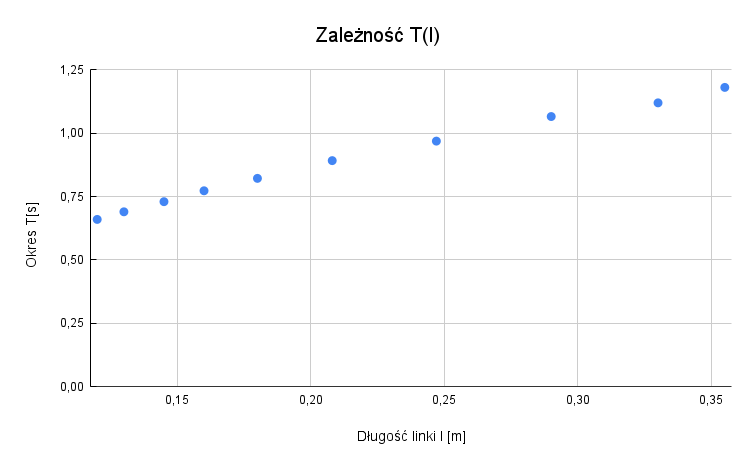
\includegraphics[width=\textwidth]{./wykres_t(l).png}
  \caption{Wykres zależności okresu drgań \(T\)
  od długości wahadła \(l\).}
  \label{fig:wykres_T(l)}
\end{figure}

\begin{figure}[H]
  \centering
  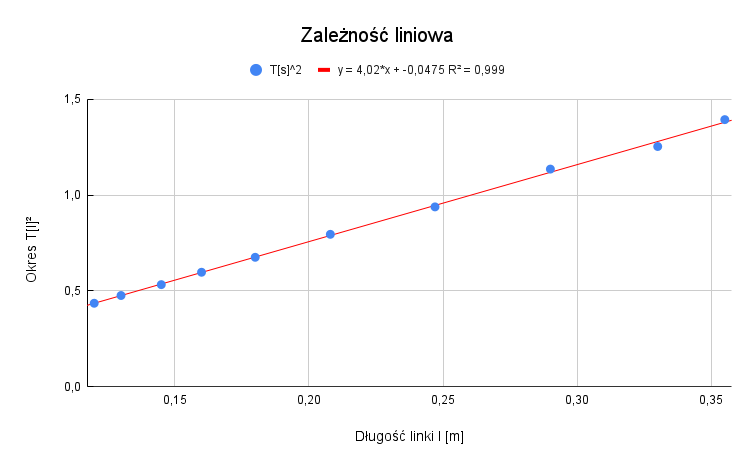
\includegraphics[width=\textwidth]{./wykres_liniowy.png}
  \caption{Wykres zależności \(T^2(l)\) z dopasowaną prostą
  metodą najmniejszych kwadratów.}
  \label{fig:wykres_liniowy}
\end{figure}

Drugi wykres okazał się liniowy, zgodny
z teoretyczną zależnością
\[
  T^2 = \frac{4\pi^2}{g}\,l + b.
\]

Dopasowanie prostej metodą najmniejszych kwadratów dało:
\[
  T^2 = (4{,}02 \pm 0{,}049)\,l - (0{,}0475 \pm 0{,}011),
\]
gdzie \(l\) wyrażono w metrach, a \(T^2\) w sekundach kwadratowych.
Otrzymany współczynnik determinacji
\(R^2 = 0{,}999\)
świadczy o bardzo dobrym dopasowaniu modelu do danych,
a niewielka wartość \(b\) wskazuje, że prosta przechodzi
blisko początku układu współrzędnych.

\pagebreak

\subsection{Wyznaczenie przyspieszenia ziemskiego}

Na podstawie nachylenia \(a\) okresowej zależności wyznaczono:
\[
  g = \frac{4\pi^2}{a}
  = \frac{4\pi^2}{4{,}02\,\frac{\text{s}^2}{\text{m}}}
  = 9{,}82\,\frac{\text{m}}{\text{s}^2}.
\]

\subsection{Niepewność i ocena zgodności}

Niepewność standardową wyznaczono z prawa przenoszenia
niepewności:
\[
  u(g) = \frac{4\pi^2}{a^2}\,u(a),
\]
przyjmując niepewność dopasowania
\(u(a) = \SI{0.049}{\second\squared\per\meter}\):
\[
  u(g) = \frac{39{,}478}{(4{,}02)^2} \cdot 0{,}049
  = \SI{0,12}{\meter\per\second\squared},
  \qquad
  U(g) = 2\,u(g) = \SI{0,24}{\meter\per\second\squared}.
\]

Ostateczny wynik:
\[
  \boxed{
    g = (9{,}82 \pm 0{,}24)\,
    \si{\meter\per\second\squared}\quad(k=2)
  }
\]

Porównując z wartością tablicową
\( g_\text{ref} = 9{,}811\,\si{m/s^2} \),
otrzymujemy różnicę
\(|g - g_\text{ref}| = 0{,}01 < U(g)\),
co oznacza, że wynik \textbf{jest zgodny} z wartością tablicową
w granicach niepewności rozszerzonej.

\subsection{Uwagi i wnioski}

Wykres \(T^2(l)\) potwierdza liniową zależność pomiędzy okresem
a pierwiastkiem z długości wahadła, zgodnie z modelem teoretycznym.
Dopasowanie prostej przez początek układu współrzędnych dało wynik
przyspieszenia ziemskiego bliski wartości tablicowej,
co świadczy o poprawnym wykonaniu pomiarów i niskim poziomie
błędów systematycznych.
Główne źródła niepewności to dokładność wyznaczenia długości
wahadła oraz reakcja mierzącego przy pomiarach czasu.
Metoda linearyzacji okazała się bardziej wiarygodna niż
wielokrotne wyznaczenie \(g\) dla jednej ustalonej długości.

\pagebreak
\section{Wnioski}

W wyniku przeprowadzonych pomiarów oraz opracowania danych
dla wahadła matematycznego wyznaczono przyspieszenie ziemskie
na dwa sposoby:
\begin{itemize}
  \item z pomiarów okresu \(T\) dla ustalonej długości \(l\):
    \[
      g_1 = (10{,}21 \pm 0{,}19)\,
      \si{\meter\per\second\squared},
    \]
  \item z pomiarów dla zmiennej długości \(l\)
    i liniowego dopasowania \(T^2(l)\):
    \[
      g_2 = (9{,}82 \pm 0{,}24)\,
      \si{\meter\per\second\squared}.
    \]
\end{itemize}

Porównanie obu wartości pokazuje, że wynik otrzymany metodą
linearyzacji jest zgodny, w granicach niepewności, z wartością
tablicową \( g_\text{ref} = 9{,}811\,\si{m/s^2} \),
natomiast wynik dla ustalonej długości wykazuje niewielkie
odchylenie (ok. 3 - 4 \%) w górę.

\bigskip
\noindent
Uzyskane rezultaty potwierdzają poprawność teoretycznego modelu
wahadła prostego, zgodnego z równaniem
\( T = 2\pi\sqrt{\frac{l}{g}} \) dla małych kątów wychylenia.
Wykres zależności \(T^2(l)\) okazała się liniowa, a współczynnik
determinacji \(R^2 = 0{,}999\) świadczy o bardzo dobrej jakości
dopasowania.

\bigskip
\noindent
Najistotniejsze źródła niepewności stanowiły:
\begin{itemize}
  \item ograniczona dokładność wyznaczenia długości \(l\)
    związana z lokalizacją środka ciężkości ciężarka,
  \item reakcja mierzącego podczas uruchamiania i zatrzymywania stopera,
  \item ewentualne drgania układu i tarcie w punkcie zawieszenia,
  \item przybliżenie \(\sin\theta \approx \theta\),
    które przestaje być ścisłe dla większych wychyleń.
\end{itemize}

Różnice między wartościami \(g_1\) i \(g_2\)
mieszczą się w realistycznych granicach błędów systematycznych
eksperymentu i nie wpływają na jakościową zgodność z teorią.
Metoda linearyzacji wykazała się większą odpornością na błędy
pojedynczych pomiarów i pozwoliła uzyskać wynik bliższy wartości
tablicowej.

\end{document}
